\documentclass[11pt]{article}
\usepackage[margin=1in]{geometry}
\usepackage{amsmath,amssymb}
\usepackage{graphicx}
\usepackage{enumitem}
\usepackage{booktabs}
\usepackage{longtable}
\usepackage{microtype}
\usepackage{hyperref}
\hypersetup{colorlinks=true,linkcolor=black,citecolor=black,urlcolor=blue}

\title{\textbf{Detection and Attribution of AI-Generated and\\
Human Written Phishing Emails from Legitimate\\
Emails Using Statistical Hypothesis Testing and\\
Naive Bayes Classifiers}}
\author{Mannan Bhardwaj -- 25BYB0013 \\ Bhoumik Singh Rajput -- 25BYB0120 \\[4pt]
School of Computer Science Engineering and Information Systems}
\date{}

\begin{document}
\maketitle

\begin{abstract}
\noindent Phishing attacks are evolving rapidly with the use of AI tools that can write convincing,
error-free emails. Most traditional filters look for human errors or simple keyword triggers,
which AI emails easily avoid. In this paper, we propose a direct, statistics-driven framework
to detect phishing emails and determine whether they were written by a human or generated
by an AI. Instead of feeding raw text directly into complex models, we extract 26 distinct
linguistic, stylistic, and structural features from each email -- 20 covering text complexity,
syntax, mechanics, communication style, and lexical richness, plus 6 added after a diagnosed
weakness in the first implementation (short legitimate emails being misread as phishing).

Every continuous feature is run through a single distribution-free difference test
(Kruskal-Wallis H), every categorical or flag feature through a Chi-Square test of independence,
and every phishing-only attribution feature through a pairwise test (Mann-Whitney U for
continuous features, a two-group Chi-Square test for categorical features). Features are kept
only if their differences are statistically significant under joint False Discovery Rate
adjustment and meet effect-size thresholds (Cohen's $d$ for continuous features, Cram\'er's $V$
for categorical features). This one-time feature-selection stage runs once on the training set
and locks its outputs -- the surviving feature list, bin edges, class-conditional frequency
tables, and class priors -- for reuse. Two specialized Naive Bayes sub-models, trained as two
entirely separate pipelines (a 3-class detector and a phishing-only 2-class attributor), are then
combined by a Meta-Naive Bayes model into a two-step decision: first, whether the email is
legitimate or phishing; second, if phishing, whether it is human-written or AI-generated.

On a held-out test set, the final pipeline reaches 86.07\% end-to-end 3-class accuracy
(86.67\% Legitimate-vs-Phishing accuracy, 98.33\% attribution accuracy). We additionally report
a controlled generalization study: training the Human-Phishing side of the pipeline on a second,
stylistically different real-world phishing corpus (419/advance-fee-fraud letters) reproduces the
same overall accuracy class but shows that detection accuracy is highly sensitive to the specific
phishing register seen during training -- a documented limitation we treat as a central finding
of this work rather than an incidental caveat.

\vspace{6pt}
\noindent\textbf{Keywords:} Phishing Detection, AI-Generated Text, Hypothesis Testing, Naive Bayes,
Feature Selection, Statistical Analysis, Stylometry, Domain Generalization.
\end{abstract}

\section{Problem Statement}
Phishing emails remain the most common entry point for cyber attacks. Historically, security
systems and human users could spot phishing messages by looking for simple clues:
\begin{enumerate}
    \item Spelling errors, broken grammar, and awkward phrasing.
    \item High-pressure urgency keywords (e.g., ``account suspended immediately'').
    \item Irregular sentence lengths and disorganized email structures.
\end{enumerate}

With modern AI text generators, these clues are no longer reliable. AI-generated phishing
emails are grammatically clean, follow standard professional formatting, and use more subtle
language. This creates two distinct challenges:
\begin{itemize}
    \item \textbf{Detection}: Differentiating between normal, legitimate emails and phishing attempts that
      contain no obvious errors.
    \item \textbf{Attribution}: Determining whether a detected phishing email was written by an individual
      human attacker or generated by an automated AI system.
\end{itemize}

Our goal is to build an interpretable system that uses clear statistical rules to solve both
challenges, providing exact mathematical reasons for every classification decision -- and, having
built it, to honestly characterize \emph{what it actually learns}, not just how well it scores on
the data it was built from.

\section{Dataset}
\label{sec:dataset}
Three labeled sources are combined into the primary dataset:
\begin{itemize}
    \item \textbf{Legitimate} email, drawn from (a) the legitimate-labeled portion of the Nazario
      corpus and (b) a raw sample from the Enron corpus, held out entirely from training and used
      only to test generalization beyond Nazario's specific legitimate-email style.
    \item \textbf{Human-Phishing}, drawn from the phishing-labeled portion of the Nazario
      corpus -- real, human-authored credential-harvesting phishing email.
    \item \textbf{AI-Phishing}, a corpus of phishing-style email generated by large language
      models across multiple model families and prompt categories, stratified-sampled to
      preserve that internal balance in training.
\end{itemize}
After deduplication and a scrub of a corpus-collection recipient address that was found to leak
class identity (Section~\ref{sec:limitations}), the primary training set is a balanced 1{,}497
emails per class (4{,}491 total); the holdout set totals 8{,}465 emails, dominated by Enron
Legitimate (4{,}934) and AI-Phishing (3{,}489), with only 42 Human-Phishing rows -- a sample-size
limitation discussed in Section~\ref{sec:generalization}. A fourth corpus, the CLAIR
advance-fee-fraud email collection (3{,}399 usable rows after cleaning), is introduced solely for
the generalization study in Section~\ref{sec:generalization} and is not part of the primary
training/evaluation split above unless explicitly stated.

\section{Proposed System Architecture}
Our methodology runs in two phases. \textbf{Phase 1 -- One-Time Feature Selection} consists of
three sequential stages -- Feature Extraction, Statistical Testing, and Feature Filtering -- executed
once on the labeled training set, and ends by locking the surviving feature list together with every
parameter the classifiers will need (bin edges, class-conditional frequency tables, class priors).
\textbf{Phase 2 -- Per-Email Classification} reuses those locked parameters to run Hierarchical
Naive Bayes Classification on any new, unlabeled email. Figure~\ref{fig:pipeline} shows the
high-level two-phase workflow; the specific refinements described in
Sections~\ref{sec:pipeline}--\ref{sec:generalization} (the length-robustness gate and the
fully-separate main/attribution pipelines) are implemented within this structure but are not yet
re-drawn into the figure.

\begin{figure}[p]
    \centering
    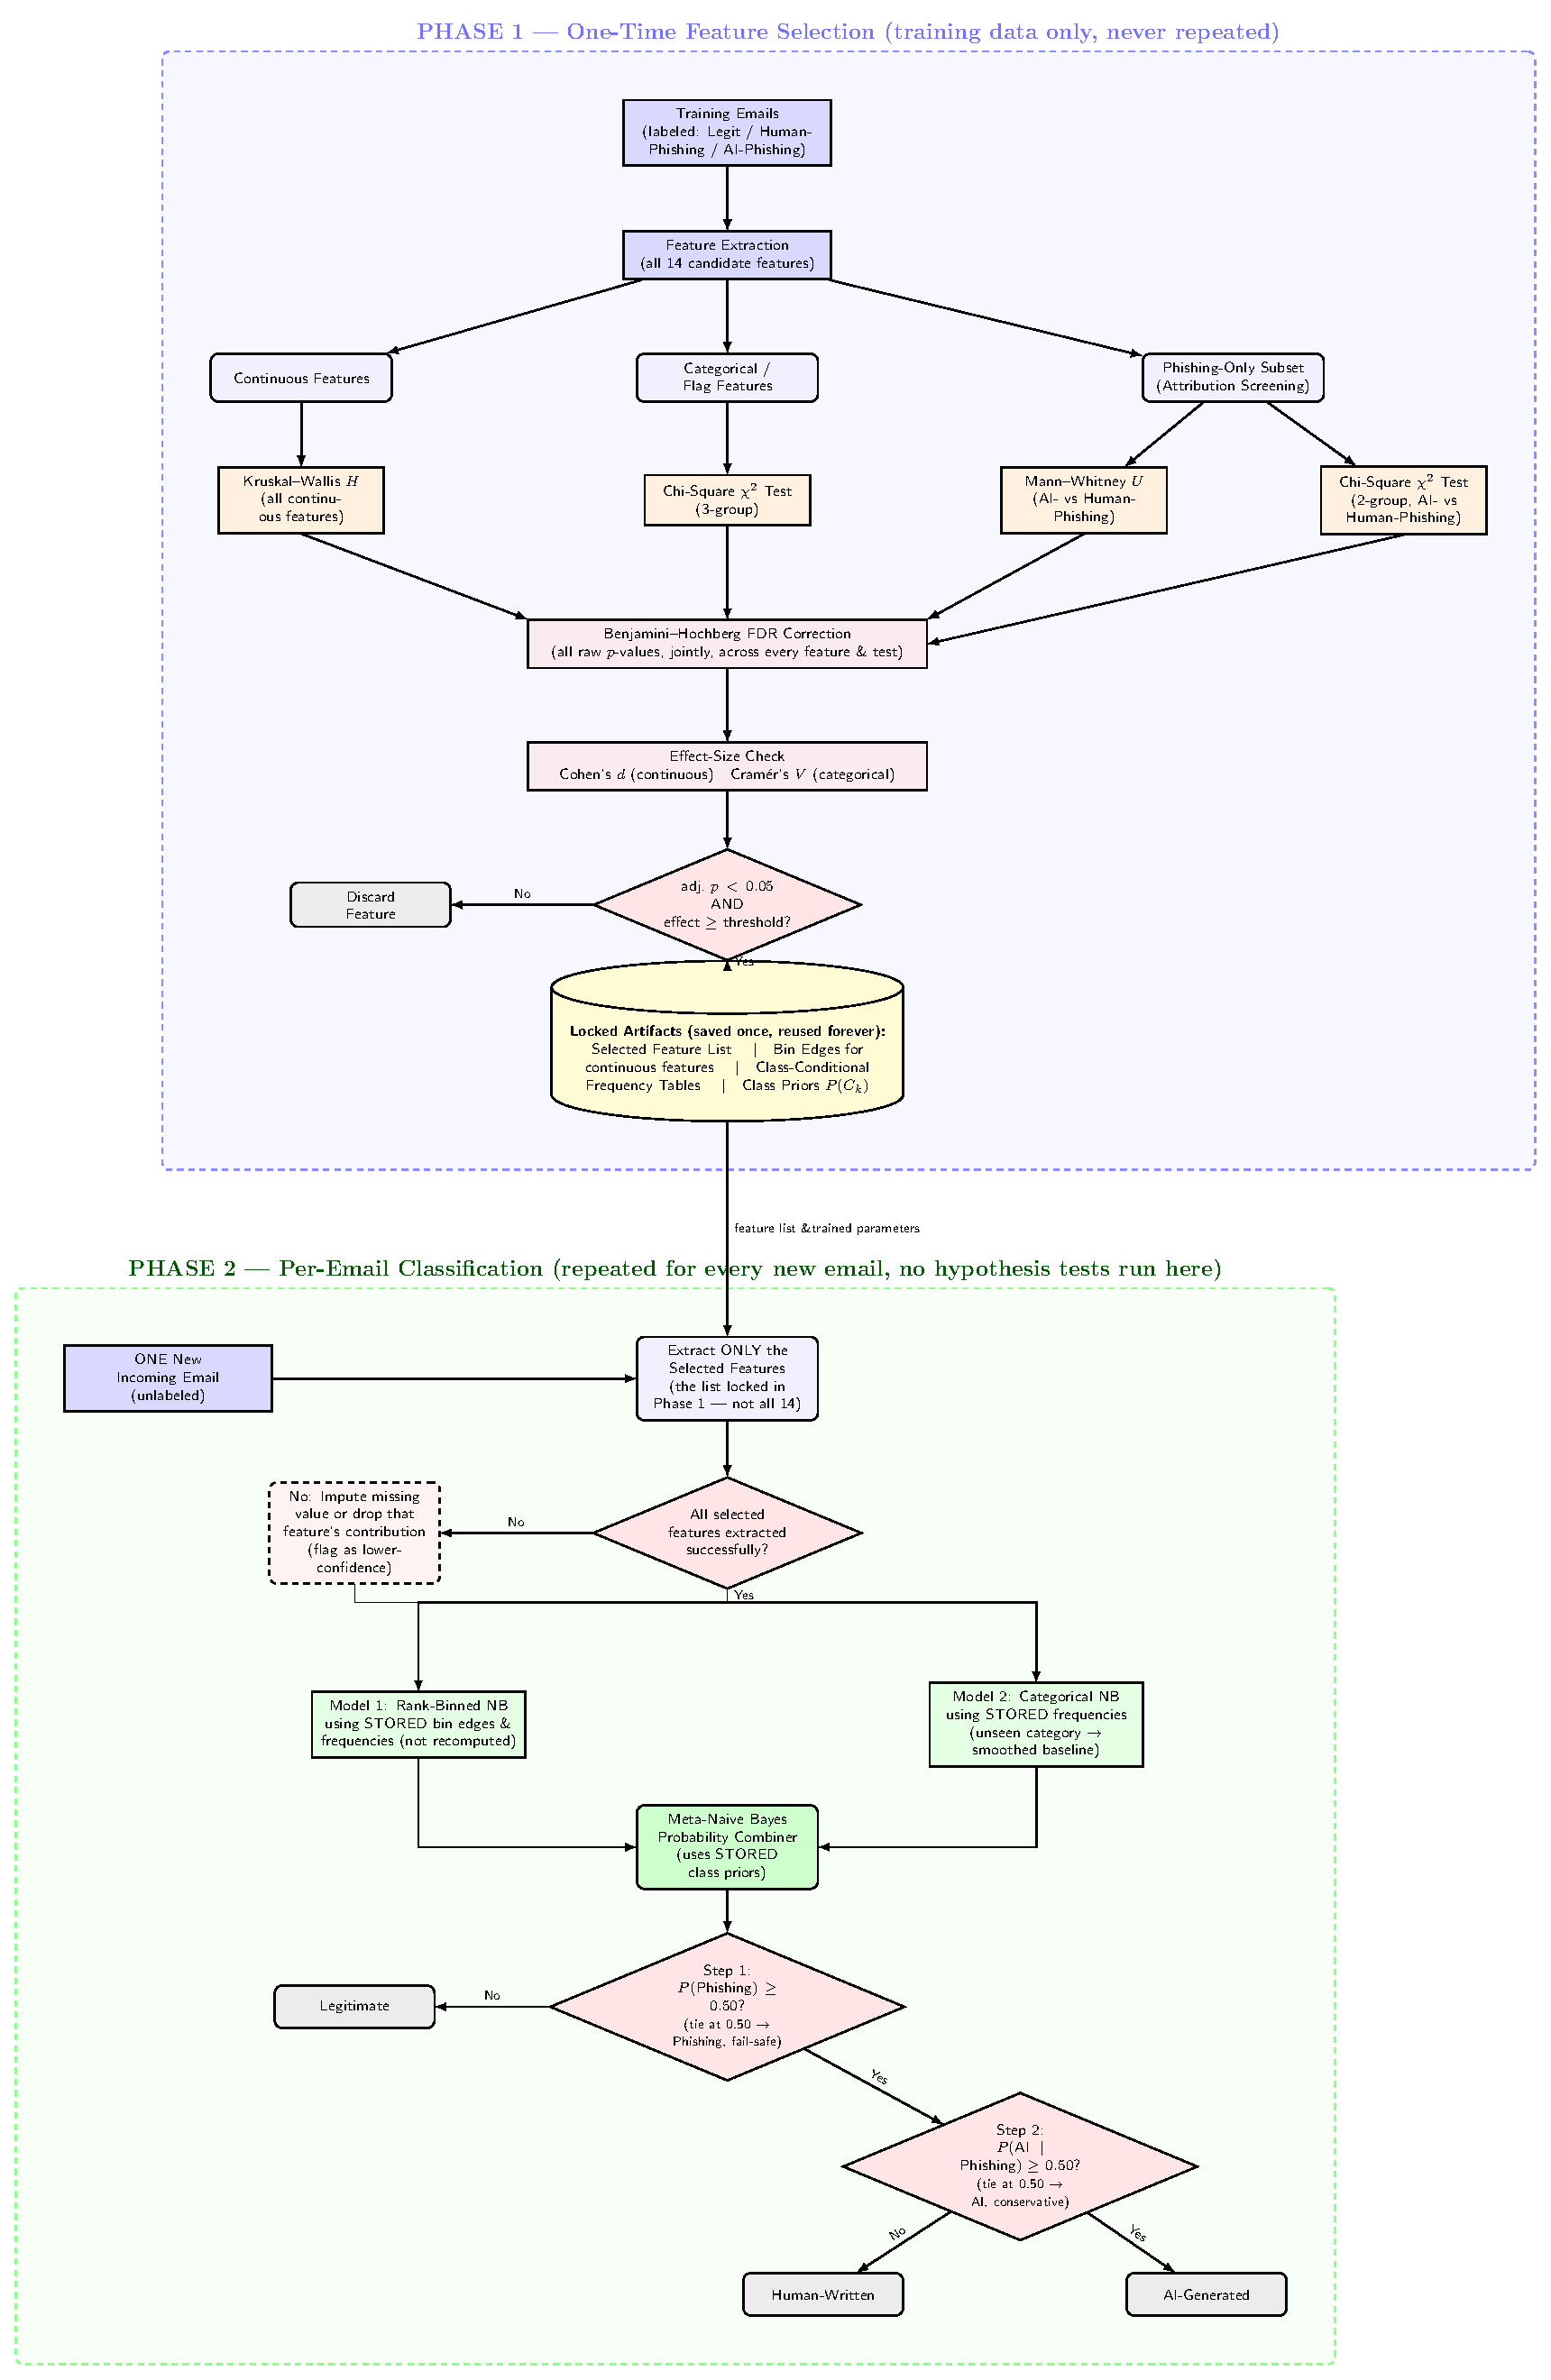
\includegraphics[width=\textwidth,height=0.85\textheight,keepaspectratio]{figure1_pipeline.pdf}
    \caption{Two-phase workflow of the feature testing and probabilistic classification pipeline.
    Phase 1 (top, blue) runs once on training data and locks its outputs into a shared parameter
    store. Phase 2 (bottom, green) classifies each new email using only those locked parameters --
    no hypothesis tests are re-run at inference time. This figure shows the general two-phase
    design; it predates the final 26-feature set, the length-robustness gate, and the
    fully-separate main/attribution pipeline split, which are described in text.}
    \label{fig:pipeline}
\end{figure}

\subsection{Linguistic Features Extracted}
We extract 26 quantifiable metrics from each email. The first 20 span five core areas:
\begin{itemize}
    \item \textbf{Text Complexity and Predictability}: Average token log-probability and sentence
      perplexity variance (burstiness), scored against a from-scratch trigram language model
      fit once on training text. AI text is typically more uniform across sentences than human
      writing.
    \item \textbf{Structure and Syntax}: Standard deviation of sentence length, maximum
      parse-tree depth, paragraph density, and clause density (linking words per sentence).
    \item \textbf{Language Mechanics}: Orthographic error density (spelling and typos) and
      punctuation distribution entropy.
    \item \textbf{Communication Style}: Density of urgency keywords, pronoun balance (ratio of
      first-person to second-person words), sentiment variance across sentences, and imperative
      verb density (e.g.\ ``click'', ``verify'', ``submit'').
    \item \textbf{Lexical Richness}: Lexical diversity (type-token ratio) and overall pronoun
      density (share of all words that are pronouns).
\end{itemize}

A further 6 features were added after diagnosing a specific failure mode of the first
implementation (Section~\ref{sec:pipeline}): several of the above features are variance or
per-100-word density measures that become near-meaningless on very short emails, causing brief
legitimate replies to resemble the ``low-variance'' signature the model associates with phishing.
The 6 additions are either presence-based (robust at any length) or explicit length signals:
\begin{itemize}
    \item \textbf{quoted\_reply\_flag}: presence of reply/quote markers (\texttt{>}, ``wrote:'',
      forwarded-header blocks) -- strong evidence of a genuine back-and-forth thread, undiluted by
      email length.
    \item \textbf{signoff\_flag}: presence of a conventional closing phrase
      (regards/thanks/sincerely/cheers) near the end of the email.
    \item \textbf{allcaps\_word\_flag}: presence of a shouted all-capitals word (excluding common
      acronyms).
    \item \textbf{multiple\_urls\_flag}: more than one distinct URL in the email.
    \item \textbf{log\_word\_count}: $\log(1+\text{word count})$, an explicit length signal that
      lets the classifier learn the length--class relationship directly rather than through a
      hand-picked threshold alone.
    \item \textbf{avg\_word\_length}: mean characters per word, a ratio rather than a raw count,
      and therefore more stable on short text.
\end{itemize}
Of these, \textbf{signoff\_flag} turned out to be the single strongest attribution signal in the
entire 26-feature set (Cram\'er's $V = 0.964$ for Human- vs.\ AI-Phishing) -- 98.3\% of AI-Phishing
training emails carry a formal sign-off versus 1.8\% of Human-Phishing emails. This supersedes an
earlier working hypothesis that imperative verb density was the strongest attribution signal; measured
against real data, imperative density's attribution effect size ($d = 0.225$) is in fact one of
the smallest that still clears the statistical gate (Section~\ref{sec:testing}).

\section{Statistical Testing Methodology}
\label{sec:testing}
Before any machine learning model sees the data, every feature must prove that its differences
between the three email groups are real and not the result of random chance. Because
email-derived linguistic features routinely violate normality (heavy skew, outliers, bounded
counts), we apply distribution-free tests directly rather than gating on a preliminary normality
check.

\subsection{Group Difference Testing}
\begin{itemize}
    \item \textbf{Kruskal-Wallis H-Test (all continuous features)}:
      \begin{equation}
        H = \frac{12}{N(N+1)} \sum_{j=1}^{k} \frac{R_j^2}{n_j} - 3(N+1)
        \label{eq:kw}
      \end{equation}
      where $R_j$ is the sum of ranks for group $j$.

    \item \textbf{Chi-Square ($\chi^2$) Test, 3-group (categorical and flag features)}:
      \begin{equation}
        \chi^2 = \sum_{i=1}^{r}\sum_{j=1}^{c} \frac{(O_{ij}-E_{ij})^2}{E_{ij}}
        \label{eq:chisq3}
      \end{equation}

    \item \textbf{Mann-Whitney U Test (Attribution, continuous features)}:
      \begin{equation}
        U = n_1 n_2 + \frac{n_1(n_1+1)}{2} - R_1
        \label{eq:mwu}
      \end{equation}

    \item \textbf{Chi-Square ($\chi^2$) Test, 2-group (Attribution, categorical features)}: the
      categorical counterpart to Mann-Whitney U, restricted to a $2 \times c$ table
      (Human-Phishing vs.\ AI-Phishing only).
\end{itemize}

\subsection{Significance and Effect Size Thresholds}
All raw $p$-values are adjusted jointly, across every feature and every test above (including
when new candidate features are added later -- see Section~\ref{sec:pipeline}), using the
Benjamini-Hochberg False Discovery Rate formula:
\begin{equation}
    P_{(i)} \leq \frac{i}{m}\cdot Q \quad (\text{with } Q = 0.05)
    \label{eq:fdr}
\end{equation}
Practical significance is additionally verified with Cohen's $d$ (continuous):
\begin{equation}
    d = \frac{\bar{x}_1 - \bar{x}_2}{s_{pooled}}, \quad
    s_{pooled} = \sqrt{\frac{(n_1-1)s_1^2 + (n_2-1)s_2^2}{n_1+n_2-2}}
    \label{eq:cohend}
\end{equation}
and Cram\'er's $V$ (categorical):
\begin{equation}
    V = \sqrt{\frac{\chi^2}{N \cdot (\min(r,c)-1)}}
    \label{eq:cramersv}
\end{equation}
Only features with adjusted $p < 0.05$ \emph{and} an effect size at or above threshold
($|d| \geq 0.20$, $V \geq 0.10$) are accepted into the classification stage -- the gate check
compares the \emph{absolute} effect size, since a large negative Cohen's $d$ is an equally strong
finding as a large positive one.

\subsection{Gate Results on the Primary (Nazario-trained) Dataset}
All 26 features clear the 3-group main gate. 20 of 26 clear the phishing-only attribution gate;
the six that fail are:
\begin{itemize}[nosep]
    \item \texttt{urgency\_density}, \texttt{pronoun\_balance}, \texttt{bracketed\_cta\_flag},
      \texttt{threat\_clause\_flag} -- significant overall but below the attribution effect-size
      threshold;
    \item \texttt{quoted\_reply\_flag}, \texttt{multiple\_urls\_flag} -- fail \emph{by design}:
      both were built to separate legitimate mail from phishing broadly, so near-zero signal once
      restricted to phishing-only rows (Human- vs.\ AI-Phishing) is the expected, correct outcome
      rather than a flaw.
\end{itemize}

\section{Probabilistic Classification Pipeline}
\label{sec:pipeline}
Features that pass Section~\ref{sec:testing} are routed into two specialized Naive Bayes models,
followed by a Meta-Naive Bayes combiner. All parameters -- bin edges, frequency tables, class
priors -- are computed once during Phase 1 and reused unchanged during Phase 2.

\subsection{Sub-Model Definitions}
\begin{itemize}
    \item \textbf{Model 1 (Rank-Binned Naive Bayes)}: continuous features, binned using
      Phase-1-locked edges:
      \begin{equation}
        P(x_i \in \text{Bin}_b \mid C_k) = \frac{N_{b,k}+\alpha}{N_k + \alpha \cdot B}
        \label{eq:rbnb}
      \end{equation}
      with Laplace smoothing $\alpha = 1$, $B=8$ quantile bins.
    \item \textbf{Model 2 (Categorical Naive Bayes)}: discrete/flag features:
      \begin{equation}
        P(x_i = v \mid C_k) = \frac{\text{Count}(x_i = v \text{ in class } C_k) + \alpha}{\text{Total samples in } C_k + \alpha \cdot K}
        \label{eq:cnb}
      \end{equation}
\end{itemize}

\subsection{Two Fully Separate Pipelines}
An ambiguity in the original design -- whether attribution reuses the main 3-class posterior or
is modeled separately -- was resolved by building \textbf{two complete, independently-trained
pipelines}: a 3-class \emph{main} pipeline (all 26 candidate features restricted to those that
clear the main gate, trained on the full balanced training set) for Step 1, and a 2-class
\emph{attribution} pipeline (restricted to attribution-gate features, trained only on
phishing-labeled training rows) for Step 2. Each pipeline fits its own Rank-Binned NB,
Categorical NB, and class priors independently.

\subsection{Length-Robustness Gate}
Investigating an elevated false-positive rate revealed that false positives were overwhelmingly
very short legitimate emails (median 22 words, versus 143 for correctly-classified legitimate
email). Four locked features are variance/spread measures that are mathematically near-zero on a
one- or two-sentence email regardless of its true class:
\begin{itemize}[nosep]
    \item \texttt{paragraph\_density}
    \item \texttt{sentence\_length\_std}
    \item \texttt{sentence\_perplexity\_variance}
    \item \texttt{sentiment\_variance}
\end{itemize}
Having verified that AI-Phishing emails are essentially never this short, we exclude these
four features from the Rank-Binned NB posterior for any email under 30 words, in both pipelines.
This is a documented \emph{partial} fix: it reduced the false-positive rate from 18.93\% to
18.14\% on the original feature set, but roughly 60\% of remaining false positives are still
short emails, indicating that several of the remaining per-100-word density features carry a
milder version of the same bias. Combined with the 6 new features above (which target the same
weakness directly), the fix becomes substantially more effective (Section~\ref{sec:results}).

\subsection{Meta-Naive Bayes Combination and Decision Steps}
\begin{equation}
    P(C_k \mid P_1, P_2) = \frac{P(C_k)\prod_{m=1}^{2} P(P_m \mid C_k)}{\sum_j P(C_j)\prod_{m=1}^{2} P(P_m \mid C_j)}
    \label{eq:metanb}
\end{equation}
\begin{enumerate}
    \item \textbf{Step 1: Phishing Detection.}
    \[ P(\text{Phishing}) = P(C_{\text{Human Phishing}}) + P(C_{\text{AI Phishing}}) \]
    If this is $< 0.50$, classify Legitimate; a tie resolves to Phishing (fail-safe).
    \item \textbf{Step 2: Threat Attribution} (only if Step 1 says Phishing).
    \[ P(\text{AI} \mid \text{Phishing}) = \frac{P(C_{\text{AI Phishing}})}{P(C_{\text{AI Phishing}}) + P(C_{\text{Human Phishing}})} \]
    If $\geq 0.50$, label AI-Generated; a tie resolves to AI-Generated (conservative).
\end{enumerate}

\section{Results}
\label{sec:results}
\begin{table}[h]
\centering
\begin{tabular}{@{}lccc@{}}
\toprule
Configuration & Step 1 acc.\ (FPR) & Step 2 acc. & End-to-end acc. \\
\midrule
20 features, no length gate & 85.43\% (18.93\%) & 86.46\% & 81.68\% \\
20 features + length gate & 85.91\% (18.14\%) & 86.46\% & 82.15\% \\
\textbf{26 features + length gate (final)} & \textbf{86.67\% (21.69\%)} & \textbf{98.33\%} & \textbf{86.07\%} \\
\bottomrule
\end{tabular}
\caption{Holdout results across the three stages of development. The final configuration is an
accepted tradeoff, not a strict improvement on every axis: overall accuracy, phishing recall
(98.36\%, up from 91.53\%), and attribution accuracy all improve substantially, but the
false-positive rate on legitimate mail rises rather than falls, because the same features that
make the model more aggressive about catching phishing also push more borderline short legitimate
emails past the detection threshold.}
\label{tab:results}
\end{table}

The large jump in Step 2 accuracy (86.46\%\,$\rightarrow$\,98.33\%) is driven almost entirely by
\texttt{signoff\_flag}. The attribution result should, however, be read with an explicit caveat:
the Human-Phishing holdout contains only 42 rows, so this figure -- while reproducible and
re-verified independently -- rests on a small sample (Section~\ref{sec:generalization} addresses
this directly by testing against a much larger second phishing corpus).

\section{Generalization Robustness Analysis}
\label{sec:generalization}
\subsection{Motivation}
The 42-row Human-Phishing holdout (Section~\ref{sec:dataset}) is too small to trust as a
generalization test on its own. We obtained a second, independent, real-world phishing corpus --
the CLAIR advance-fee-fraud (``419 scam'') email collection -- specifically to grow this sample.
After cleaning (removing 3 corrupted mbox-artifact rows and 573 internal duplicates, and verifying
zero cross-corpus duplication with the existing dataset), 3{,}399 usable rows remained.

\subsection{First Test: Same Model, Larger Holdout}
Adding these 3{,}399 rows purely to the holdout set (training untouched) and re-scoring the
already-accepted model (Table~\ref{tab:results}, final row) produced a sharp drop: Step 1
accuracy fell from 86.67\% to 65.46\%, and end-to-end accuracy from 86.07\% to 64.99\%. Splitting
the Human-Phishing holdout by source isolates the cause precisely:
\begin{center}
\begin{tabular}{@{}lcc@{}}
\toprule
Human-Phishing holdout subset & $n$ & caught as phishing at all \\
\midrule
Nazario-style (seen during training) & 42 & 100.0\% \\
CLAIR-style (never seen during training) & 3{,}399 & 12.6\% \\
\bottomrule
\end{tabular}
\end{center}
A feature-level comparison explains why: CLAIR's advance-fee-fraud letters are long narrative
appeals (mean 508 words, versus 131 for Nazario-phishing) that almost entirely lack the
credential-harvesting markers the locked feature set relies on -- urgency language (23.5\% vs.\
38.2\%), sensitive-information requests (6.9\% vs.\ 7.1\%), threat clauses (8.5\% vs.\ 23.8\%),
and generic greetings (4.9\% vs.\ 9.5\%) are all markedly rarer, while \texttt{quoted\_reply\_flag}
-- a feature explicitly designed to indicate \emph{legitimate} correspondence -- fires on 9.4\% of
CLAIR phishing, far above its phishing-class baseline.

\subsection{Second Test: A Fully Retrained, Symmetric Ablation}
To confirm this is a property of training distribution rather than a quirk of one model, we
retrained the Human-Phishing side of the pipeline \emph{entirely} on the CLAIR corpus (Legitimate
and AI-Phishing training left completely unchanged, re-running the full statistical gate and both
Naive Bayes pipelines from scratch). The result mirrors the first test in reverse:
\begin{center}
\begin{tabular}{@{}lccc@{}}
\toprule
Trained on & Tested on & $n$ & Caught as phishing \\
\midrule
Nazario & Nazario (same style) & 42 & 100.0\% \\
Nazario & CLAIR (different style) & 3{,}399 & 12.6\% \\
CLAIR & CLAIR (same style) & 1{,}902 & 87.1\% \\
CLAIR & Nazario (different style) & 42 & 2.4\% \\
\bottomrule
\end{tabular}
\end{center}
The CLAIR-trained model's higher headline accuracy (93.78\% end-to-end; 5.35\% false-positive
rate) is \emph{not} evidence that it generalizes better -- it reflects that CLAIR's long narrative
letters are more structurally distinct from Enron business email than Nazario's phishing is, not
an improvement in the model's concept of ``phishing.'' Whichever corpus supplies training data,
the pipeline learns that corpus's specific phishing register and transfers it poorly to the other.

\subsection{Interpretation}
\label{sec:limitations}
We treat this symmetric result as the central methodological finding of the generalization study,
not an incidental limitation to be minimized. The 26-feature set, however statistically validated
within one register, implicitly encodes a credential-harvesting-style definition of ``phishing''
(urgency, fake-login prompts, sensitive-information requests) when trained on Nazario, and a
narrative-fraud-style definition when trained on CLAIR; it does not yet capture a
register-independent notion of phishing intent. Two further points are worth recording
transparently: a corpus-collection recipient address (\texttt{jose@monkey.org}) was found to leak
class identity directly into Human-Phishing email bodies and was removed by deletion (not
placeholder substitution, which would simply relocate the leak) before any result in this paper
was produced; and the AI-Phishing corpus concentrates a small number of fake domains at near-100\%
within that class, confirmed by an independent TF-IDF/logistic-regression check to carry genuine
predictive signal rather than being an artifact, but still a template-reuse characteristic worth
flagging for future dataset expansion.

\section{Summary of System Characteristics}
\begin{enumerate}
    \item \textbf{Direct Statistical Gating}: Features are included only after clearing formal
      hypothesis testing with joint multiple-comparison correction.
    \item \textbf{Full Auditability}: Every classification can be traced back to exact feature
      likelihoods and probability scores -- no black-box component is involved.
    \item \textbf{Low Compute Overhead}: Naive Bayes inference over pre-locked parameters enables
      fast per-email classification without specialized hardware.
    \item \textbf{Train-Once, Classify-Many Separation}: Every hypothesis test, bin edge, and
      frequency table is computed exactly once during Phase 1.
    \item \textbf{Documented Generalization Scope}: Rather than reporting a single accuracy figure
      as unconditionally generalizable, we explicitly characterize the register-specific nature of
      what the feature set learns, backed by a controlled, symmetric ablation
      (Section~\ref{sec:generalization}).
\end{enumerate}

\section{Limitations and Future Work}
The attribution result rests on a small same-style holdout (42 rows); the generalization study
mitigates but does not eliminate this, since each individual retrained model still sees only one
phishing register during training. A natural next step is a mixed-register training set (Nazario
and CLAIR combined) to test whether the pipeline can learn a broader notion of phishing rather
than a single register, and whether doing so costs same-register accuracy. The length-robustness
gate and the 6 new features reduce, but do not eliminate, the short-email false-positive problem;
a more principled length-normalization scheme for the remaining per-100-word density features is
left as future work.

\end{document}
